\documentclass[11pt]{article}

\newcommand{\yourname}{Zerun Tian}
\newcommand{\yourcollaborators}{}

\def\comments{0}
\setlength{\parindent}{0 in}
\setlength{\parskip}{0.1in}

\usepackage{graphicx}
\graphicspath{ {./} }

%format and packages

%\usepackage{algorithm, algorithmic}
\usepackage[noend]{algpseudocode}
\usepackage{amsmath, amssymb, amsthm}
\usepackage{enumerate}
\usepackage{enumitem}
\usepackage{framed}
\usepackage{verbatim}
\usepackage[margin=1.0in]{geometry}
\usepackage{microtype}
\usepackage{kpfonts}
\usepackage{palatino}
	\DeclareMathAlphabet{\mathtt}{OT1}{cmtt}{m}{n}
	\SetMathAlphabet{\mathtt}{bold}{OT1}{cmtt}{bx}{n}
	\DeclareMathAlphabet{\mathsf}{OT1}{cmss}{m}{n}
	\SetMathAlphabet{\mathsf}{bold}{OT1}{cmss}{bx}{n}
	\renewcommand*\ttdefault{cmtt}
	\renewcommand*\sfdefault{cmss}
	\renewcommand{\baselinestretch}{1.06}
\usepackage[usenames,dvipsnames]{xcolor}
\definecolor{DarkGreen}{rgb}{0.15,0.5,0.15}
\definecolor{DarkRed}{rgb}{0.6,0.2,0.2}
\definecolor{DarkBlue}{rgb}{0.2,0.2,0.6}
\definecolor{DarkPurple}{rgb}{0.4,0.2,0.4}
\usepackage[pdftex]{hyperref}
\hypersetup{
	linktocpage=true,
	colorlinks=true,				% false: boxed links; true: colored links
	linkcolor=DarkBlue,		% color of internal links
	citecolor=DarkBlue,	% color of links to bibliography
	urlcolor=DarkBlue,		% color of external links
}


%enclosure macros
\newcommand{\paren}[1]{\ensuremath{\left( {#1} \right)}}
\newcommand{\bracket}[1]{\ensuremath{\left\{ {#1} \right\}}}
\renewcommand{\sb}[1]{\ensuremath{\left[ {#1} \right\]}}
\newcommand{\ab}[1]{\ensuremath{\left\langle {#1} \right\rangle}}

%probability macros
\newcommand{\ex}[2]{{\ifx&#1& \mathbb{E} \else \underset{#1}{\mathbb{E}} \fi \left[#2\right]}}
\newcommand{\pr}[2]{{\ifx&#1& \mathbb{P} \else \underset{#1}{\mathbb{P}} \fi \left[#2\right]}}
\newcommand{\var}[2]{{\ifx&#1& \mathrm{Var} \else \underset{#1}{\mathrm{Var}} \fi \left[#2\right]}}

%useful CS macros
\newcommand{\poly}{\mathrm{poly}}
\newcommand{\polylog}{\mathrm{polylog}}
\newcommand{\zo}{\{0,1\}}
\newcommand{\pmo}{\{\pm1\}}
\newcommand{\getsr}{\gets_{\mbox{\tiny R}}}
\newcommand{\card}[1]{\left| #1 \right|}
\newcommand{\set}[1]{\left\{#1\right\}}
\newcommand{\negl}{\mathrm{negl}}
\newcommand{\eps}{\varepsilon}
\DeclareMathOperator*{\argmin}{arg\,min}
\DeclareMathOperator*{\argmax}{arg\,max}
\newcommand{\eqand}{\qquad \textrm{and} \qquad}
\newcommand{\ind}[1]{\mathbb{I}\{#1\}}
\newcommand{\sslash}{\ensuremath{\mathbin{/\mkern-3mu/}}}

%mathbb
\newcommand{\N}{\mathbb{N}}
\newcommand{\R}{\mathbb{R}}
\newcommand{\Z}{\mathbb{Z}}
%mathcal
\newcommand{\cA}{\mathcal{A}}
\newcommand{\cB}{\mathcal{B}}
\newcommand{\cC}{\mathcal{C}}
\newcommand{\cD}{\mathcal{D}}
\newcommand{\cE}{\mathcal{E}}
\newcommand{\cF}{\mathcal{F}}
\newcommand{\cL}{\mathcal{L}}
\newcommand{\cM}{\mathcal{M}}
\newcommand{\cO}{\mathcal{O}}
\newcommand{\cP}{\mathcal{P}}
\newcommand{\cQ}{\mathcal{Q}}
\newcommand{\cR}{\mathcal{R}}
\newcommand{\cS}{\mathcal{S}}
\newcommand{\cU}{\mathcal{U}}
\newcommand{\cV}{\mathcal{V}}
\newcommand{\cW}{\mathcal{W}}
\newcommand{\cX}{\mathcal{X}}
\newcommand{\cY}{\mathcal{Y}}
\newcommand{\cZ}{\mathcal{Z}}

%theorem macros
\newtheorem{thm}{Theorem}
\newtheorem{lem}[thm]{Lemma}
\newtheorem{fact}[thm]{Fact}
\newtheorem{clm}[thm]{Claim}
\newtheorem{rem}[thm]{Remark}
\newtheorem{coro}[thm]{Corollary}
\newtheorem{prop}[thm]{Proposition}
\newtheorem{conj}[thm]{Conjecture}

\theoremstyle{definition}
\newtheorem{defn}[thm]{Definition}


\newcommand{\instructor}{Virgil Pavlu}
\newcommand{\hwnum}{6}
\newcommand{\hwdue}{Wednesday, May 20 at 11:59pm via \href{https://gradescope.com/courses/229309}{Gradescope}}

\theoremstyle{theorem}
\newtheorem{prob}{}
\newtheorem{sol}{Solution}

\definecolor{cit}{rgb}{0.05,0.2,0.45} 
\newcommand{\solution}{\medskip\noindent{\color{DarkBlue}\textbf{Solution:}}}

\begin{document}
{\Large 
\begin{center}{CS5800: Algorithms} --- Spring '21 --- \instructor \end{center}}
{\large
\vspace{10pt}
\noindent Homework~\hwnum \vspace{2pt}\\
Submit via \href{https://www.gradescope.com/courses/232127}{Gradescope}}

\bigskip
{\large \noindent Name: \yourname }

{\large \noindent Collaborators: \yourcollaborators}

\vspace{15pt}

{\large \noindent Instructions:}

\begin{itemize}

\item Make sure to put your name on the first page.  If you are using the \LaTeX~template we provided, then you can make sure it appears by filling in the \texttt{yourname} command.

\item Please review the grading policy outlined in the course information page.

\item You must also write down with whom you worked on the assignment.  If this changes from problem to problem, then you should write down this information separately with each problem.

\item Problem numbers (like Exercise 3.1-1) are corresponding to CLRS $3^{rd}$ edition.  While the  $2^{nd}$ edition  has  similar  problems  with  similar  numbers,  the  actual  exercises  and their solutions are different, so make sure you are using the $3^{rd}$ edition.

\end{itemize}

%%% Problem 1 %%%
\newpage
\begin{prob} \textbf{(40 points + Extra Credit 40 points)}
\end{prob}
Jars on a ladder problem.  Given a ladder of $n$ rungs and $k$ identical glass jars,  one has to design an experiment of dropping jars from certain rungs, in order to find the highest rung (HS) on the ladder from which a jar doesn’t break if dropped.

Idea: With only one jar ($k=1$), we can’t risk breaking the jar without getting an answer. So we start from the lowest rung on the ladder, and move up.  When the jar breaks, the previous rung is the answer; if we are unlucky, we have to do all n rungs, thus n trials. Now lets think of $k=\log(n)$:  with $\log(n)$ or more jars, we have enough jars to do binary search,  even  if  jars  are  broken  at  every  rung. So  in  this  case  we  need  $\log(n)$  trials. Note  that  we  can’t  do  binary  search  with  less  than  $\log(n)$  jars,  as  we  risk  breaking  all jars before arriving at an answer in the worst case.

Your task is to calculate \textit{q = MinT(n, k)} = the minimum number of dropping trials any such experiment has to make, to solve the problem even in the worst/unluckiest case (i.e., not running out of jars to drop before arriving at an answer). \textit{MinT} stands for Minimum number of Trials.

%%% Problem 1.a %%%
\noindent\textbf{A(5 points).} Explain the optimal solution structure and write a recursion for $\textit{MinT}(n, k)$. 

\solution

Suppose we are given an optimal solution that finds the highest rung (HS) $m$ using $q$ dropping trails. If we drop a jar at any intermediate rung $x$, there are two results: either it breaks or doesn't break. When it breaks, we need to test for $x-1$ number of rungs that are below $x$ with one less jar $k - 1$. On the other hand, we need to test for $n - x$ number of rungs that are above $x$ with the same $k$ number of jars. 
We define the following recursion,
\[
\textit{MinT}(n, k) = 
\begin{cases}
	0 &\mbox{if } k = 0 \\
	n &\mbox{if } n  \le 1 \text{ or } k = 1 \\
	1 + \min_{1 \le x \le n} \Big\{ \max \big\{ \textit{MinT}(x - 1, k - 1),  \textit{MinT}(n - x, k) \big\} \Big\} 	&\mbox{if } n > 1 \text{ and } k > 1 
\end{cases}
\]

Specifically, we simulate dropping a jar from every rung and find the minimum number of trails among them. For every dropping test, the jar will either break or survive. A broken jar implies a subproblem of $x-1$ floors with $k-1$ jars. On the other hand, a survived jar implies a subproblem of $n-x$ remaining floors with $k$ jars. We choose whichever is larger as we are considering the worst case scenario. In the end, we must have covered the $(m+1)$-th rung where a jar broke and covered the first $m-1$ number of rungs in $q-1$ trails where jars didn't break. 


\newpage
%%% Problem 1.b %%%
\noindent\textbf{B(5 points).} Write  the  alternative/dual  recursion for $\textit{MaxR}(k, q)$  =  the Highest Ladder Size $n$ doable with $k$ jars and maximum $q$ trials.  Explain how $\textit{MinT}(n, k)$ can be computed from the table $\textit{MaxR}(k, q)$. \textit{MaxR} stands for the Maximum number of Rungs.

\solution

Here is the recursion for the reformulated problem,
\[
\textit{MaxR}(k, q) =
\begin{cases}
	0 &\mbox{if } k = 0 \\
	q &\mbox{if } k = 1 \text{ or } q \le 1 \\
	1 + \textit{MaxR}(k - 1, q - 1) + \textit{MaxR}(k, q - 1) &\mbox{if } k > 1 \text{ and } q > 1
\end{cases}
\]
When we have only one jar, the highest ladder size we can possibly test is $q$. For more than one jar, the highest ladder size is a combination of solutions to subproblem of $k-1$ jars (the jar at trial $q$ broke) and subproblem of $k$ jars (the jar did not broke) with $q-1$ trails. We can figure out $\textit{MinT}(n, k)$ by looking at the $k$-th row of the table $\textit{MaxR}(k, q)$ and find a cell whose value is no less than and the closest to $n$. The column number of that cell represents the minimum number of trails we need for $\textit{MinT}(n, k)$.

\newpage
%%% Problem 1.c %%%
\noindent\textbf{C(10 points).} For one of these two recursions (not both, take your pick) write the bottom-up non-recursive computation pseudocode. \textit{Hint:  the recursion MinT(n, k) is a bit more difficult and takes more computation steps, but once the table is computed, the rest is easier on points E-F below.  The recursion in MaxR(q, k) is perhaps easier, but trickier afterwards:  make sure you compute all cells necessary to get MinT(n, k) — see point B.}

\solution

Let's write the pseudocode for $\textproc{\textsc{MinT}}(n, k)$,

\begin{algorithmic}[1]
\Function{MinT}{$n$, $k$}
	\State let $C[0..n, 0..k]$ and $S[0..n, 0..k]$ be tables of zeros \Comment{table initializations}
	\For {$i = 0$ \text{to} $k$}
		\State $C[1, i] = 1$
	\EndFor
	\For {$i = 0$ \text{to} $n$}
		\State $C[i, 1] = i$
	\EndFor
	
	\For {$i = 2$ \text{to} $n$} 	\Comment{filling the table}
		\For {$j = 2$ \text{to} $k$}
			\State $C[i, j] = +\inf$
			\For {$x = 1$ \text{to} $i$}
				\State $\textit{cost} = \text{max}(C[x - 1, j - 1], C[i - x, j])$
				\If {$\textit{cost} < C[i, j]$}
					\State $C[i, j] = \textit{cost}$
					\State $S[i, j] = x$
				\EndIf
			\EndFor
			\State $C[i, j] = C[i, j] + 1$
		\EndFor
	\EndFor
	\State \textbf{return} $C$, $S$
\EndFunction
\end{algorithmic}


\newpage
%%% Problem 1.d %%%
\noindent\textbf{D(10 points).} Redo the computation this time top-down recursive, using memoization.

\solution

\begin{algorithmic}[1]
\Function{MemoizedMinT}{$n$, $k$}
	\State let $C[0..n, 0..k]$ be a table of negative ones and $S[0..n, 0..k]$ be a table of zeros
	\For {$i = 0$ \text{to} $k$}
		\State $C[0, i] = 0$
		\State $C[1, i] = 1$
	\EndFor
	\For {$i = 0$ \text{to} $n$}
		\State $C[i, 0] = 0$
		\State $C[i, 1] = i$
	\EndFor
	\State \textbf{return} $\textproc{\textsc{Helper}}(n$, $k$, $C$, $S)$
\EndFunction
\end{algorithmic}

\begin{algorithmic}[1]
\Function{Helper}{$n$, $k$, $C$, $S$}
	\If {$n \le 1$ or $k \le 1$}
		\State \textbf{return} $C[n, k]$
	\EndIf
	\State \textit{minCost} $= $ +inf
	\For {$x =$ 1 to $n$}
		\State $\textit{broke} = C[x-1][k-1]$
		\If {$\textit{broke} == -1$}
			\State $\textit{broke} = \textproc{\textsc{Helper}}(x-1$, $k-1$, $C$, $S)$
			\State $C[x-1, k-1] = \textit{broke}$
		\EndIf
		\State $\textit{survived} = C[n - x][k]$
		\If {$\textit{survived} == -1$}
			\State $\textit{survived} = \textproc{\textsc{Helper}}(n - x$, $k$, $C$, $S)$
			\State $C[n-x, k] = \textit{survived}$
		\EndIf
		\State $\textit{cost} = \text{max}(\textit{broke}$, $\textit{survived})$
		\If {$\textit{cost} < \textit{minCost}$}
			\State $\textit{minCost} = \textit{cost}$
			\State $C[n, k] = \textit{minCost}$
			\State $S[n, k] = x$
		\EndIf
	\EndFor
	\State \textbf{return} $\textit{minCost} + 1$
\EndFunction
\end{algorithmic}


\newpage
%%% Problem 1.e %%%
\noindent\textbf{E(10 points).} Trace  the  solution.   While  computing  bottom-up,  use  an  auxiliary structure  that  can  be  used  to  determine  the  optimal  sequence  of  drops  for  a  given input n, k.  The procedure TRACE(n, k) should output the ladder rungs to drop jars, considering the dynamic outcomes of previous drops. \textit{Hint:  its recursive.  Somewhere in the procedure there should be an if statement like “if the trial at rung x breaks the jar...  else ...”}

\solution

We define the following recursive procedure to trace a solution under different outcomes at every trail. The last argument $b$ of \textproc{\textsc{Trace}} represents the beginning rung in order to offset correctly. To generate a solution string, we simply call $\textproc{\textsc{Trace}}(S$, $n$, $k$, $0)$.
\begin{algorithmic}[1]
\Function{Trace}{$S$, $n$, $k$, $b$}
	\If {$S[n][k] == 0$}
		\State \textbf{return} "If jar breaks at rung " + $(b + n)$ + ": HS is " +  $b$ + " else HS is " + $(b+n)$
	\EndIf
	\State \textit{rung} $= b + S[n][k]$
	\State $\textit{out} =$ "If jar breaks at rung " + \textit{rung}
	\State $\textit{out} = \textit{out } + $ ": do linear search from " + $(b + S[n][k-1] + 1)$ + " to " + $(\textit{rung} - 1)$ +  \textbackslash n  
	\State $\textit{out} = \textit{out } + $ "else " + \textproc{\textsc{Trace}}$(S$, $n - S[n][k]$, $k$, $\textit{rung})$
	\State \textbf{return} \textit{out}
\EndFunction
\end{algorithmic}

\newpage
%%% Problem 1.f (EC) %%%
\noindent\textbf{F(extra credit, 20 points).} Output  the  entire  decision  tree  from  part  E)  using JSON  to  express  the  tree,  for  the  following  test  cases : (n=9,k=2); (n=11,k=3); (n=10000,k=9). Turn in your program that produces the optimum decision tree for given n and k using JSON as described below.  Turn in a zip folder that contains:  (1) all files required by your program (2) instructions how to run your program (3) the three decision trees in files t-9-2.txt, t-11-3.txt and t-10000-9.txt (4) the answers to all other questions of this homework.

To represent an algorithm, i.e., an experimental plan, for finding the highest safe rung for fixed n,k, and q we use a restricted programming language that is powerful enough to express what we need.  We use the programming language of binary decision trees which  satisfy  the  rules  of  a  binary  search  tree.   The  nodes  represent  questions  such as 7 (representing the question:  does the jar break at rung 7?).  The edges represent yes/no answers.  We use the following simple syntax for decision trees based on JSON. The reason we use JSON notation is that you can get parsers from the web and it is a widely used notation.  A decision tree is either a leaf or a compound decision tree represented by an array with exactly 3 elements

\begin{verbatim}
// h = highest safe rung or leaf
{ "decision_tree" : [1,{"h":0},[2,{"h":1},[3,{"h":2},{"h":3}]]] }
\end{verbatim}

\noindent The grammar and object structure would be in an EBNF-like notation:

\begin{verbatim}
DTH = "{" "\"decision_tree\"" ":" <dt> DT.
DT = Compound | Leaf.
Compound = "[" <q> int "," <yes> DT "," <no> DT "]".
Leaf = "{" "\"h\" " ":" <leaf> int "}".
\end{verbatim}

\noindent This approach is useful for many algorithmic problems:  define a simple computational model in which to define the algorithm.  The decision trees must satisfy certain rules to be correct.
\\ \\
\noindent A decision tree t in DT for HSR(n,k,q) must satisfy the following properties:

(a)  the  BST  (Binary  Search  Tree  Property):  For  any  left  subtree:  the  root  is  one larger than the largest node in the subtree and for any right subtree the root is equal to the smallest (i.e., leftmost) node in the subtree.

(b)  there are at most k yes from the root to any leaf.

(c)  the longest root-leaf path has q edges.

(d)  each rung 1..n-1 appears exactly once as internal node of the tree.

(e)  each rung 0..n-1 appears exactly once as a leaf.
\\

\noindent If all properties are satisfied, we say the predicate correct(t,n,k,q) holds.  HSR(n,k,q) returns a decision tree t so that correct(t,n,k,q).
\\

\noindent To test your trees, you can download the JSON HSR-validator from the url:

\noindent\texttt{https://github.com/czxttkl/ValidateJsonDecisionTree}
\\

%%% Problem 1.g (EC) %%%
\noindent\textbf{G(extra credit, 20 points).} Solve a variant of this problem for q= MinT(n,k) that optimizes the average case instead of the worst case:  now we are not concerned with the worst case q, but with the average q.  Will make the assumption that all cases are equally likely (the probability of the answer being a particular rung is the same for all rungs).  You will have to redo points A,C,E specifically for this variant.


\newpage
%%% Problem 2 %%%
\begin{prob} \textbf{(20 points)} Problem 15-2.  Hint:  try to use the LCS problem as a procedure.
\end{prob}

Give an efficient algorithm to find the longest palindrome that is a subsequence of a given input string. What is the running time of your algorithm?

\solution

Let's call the input string $X$ and create a string $Y$ that is the input string reversed. We can now apply the DP procedure of \textit{LCS} to find the longest common subsequence $S$ between $X$ and $Y$. We claim that $S$ is the longest palindrome of $X$. Suppose there exists a longer palindrome $S'$ in $X$. We are guaranteed to find $S'$ in $Y$ because $Y$ is $X$ reversed and $S'$ reversed is $S'$. The \textit{LCS} procedure should have produced $S'$ as the longest common subsequence instead of $S$. This contradiction shows our claim is correct. 

Producing a string $Y$ takes $O(n)$-time where n is the length of the input string $X$. DP solution to \textit{LCS} runs in $O(mn)$-time where $m$ and $n$ are the sizes of the two input strings. Running \textit{LCS} on our $X$ and $Y$ takes $O(n^2)$-time because both are length $n$. Overall, the algorithm runs in $O(n^2)$-time.


\newpage
%%% Problem 3 %%%
\begin{prob} \textbf{(30 points)} Exercise 15.4-6.
\end{prob}

Give an $O(n\lg n)$-time algorithm to find the longest monotonically increasing subsequence of a sequence of $n$ numbers.

\solution

\begin{enumerate}[label=(\arabic*)]
\item Characterize the structure of an optimal solution:

Suppose we are given a sequence $A = [a_1, a_2, ..., a_k]$ that is the longest monotonically increasing subsequence (LMIS) of the original sequence $X = [x_1, x_2, ..., x_n]$ of $n$ numbers. We make following observations:

1. If $x_n = a_k$, then $A_{k-1}$ is the LMIS of $X_{n-1}$. \\
2. If $x_n \ne a_k$, then $A$ is the LMIS of $X_{n-1}$.

\item Define the recurrence of the objective:

We fill an auxiliary array $S[0..n]$ with every value $x_i$ by finding a $k$ such that $S[k] < x_i < S[k+1]$, then replacing $S[k+1]$ with $x_i$. The resulting $S$ maintains that $S[i]$ is the smallest last value of the monotonically increasing subsequence of length $i$. We notice that $S$ is sorted at every step. In the meantime, in $C[0..n]$, we keep track of the monotonically increasing subsequence of different length whose last value is the smallest possible so far. This is achieved by setting $C[k+1] = C[k] + [x_i]$.

\item Compute the value of an optimal solution bottom-up:

\begin{algorithmic}[1]
\Function{FindLMIS}{$X$}
	\State let $C[0..n]$ be an array of empty arrays
	\State let $S[0..n]$ be an auxiliary array of $+\infty$
	\State $l = 0$
	\For {$i = 1$ to $n$}
		\Comment{do binary search on $S$ to find a $k$}			
		\State $k = \text{search } S[k] < X[i] < S[k+1]$ or $0$ \Comment{assign $k$ to 0 if $X[i] \le S[k]$ for all $k$}
		\State $S[k + 1] = X[i]$
		\State $C[k + 1] = C[k] + [X[i]]$
		\If {$k + 1 > l$}
			\State $l = k + 1$ 
		\EndIf
	\EndFor
	\State \textbf{return} $C[l]$
\EndFunction
\end{algorithmic}


\item Trace the optimal solution from the computed information:

The optimal solution is directly returned by $\textproc{\textsc{FindLMIS}}$.

\item Runtime and space requirements:

During each iteration of the loop, the binary search operation at line 6 costs $O(\lg n)$-time, remaining operations cost $O(1)$-time, so each iteration takes $O(\lg n)$-time. There are $n$ iterations, so the runtime of the algorithm is $O(n \lg n)$. The algorithm requires $O(n)$ space for storing the $C$ and $S$ one-dimensional arrays of size $n+1$.

\end{enumerate}



\newpage
%%% Problem 4 %%%
\begin{prob} \textbf{(Extra Credit 20 points)} 
\end{prob}

Suppose that you are the curator of a large zoo.  You have just received a grant of $\$m$ to purchase new animals at an auction you will be attending in Africa.  There will be an essentially unlimited supply of $n$ different types of animals, where  each  animal  of  type $i$ has  an  associated  cost $c_i$.   In  order  to  obtain  the  best possible selection of animals for your zoo, you have assigned a value $v_i$ to each animal type, where $v_i$ may be quite different than $c_i$.  (For instance, even though panda bears are quite rare and thus expensive,  if your zoo already has quite a few panda bears, you might associate a relatively low value to them.)  Using a business model, you have determined that the best selection of animals will correspond to that selection which maximizes  your  perceived  profit  (total  value  minus  total  cost);  in  other  words,  you wish to maximize the sum of the profits associated with the animals purchased. Devise an efficient algorithm to select your purchases in this manner.  You may assume that $m$ is a positive integer and that $c_i$ and $v_i$ are positive integers for all i.  Be sure to analyze the running time and space requirements of your algorithm.

\solution

\newpage
%%% Problem 5 %%%
\begin{prob} \textbf{(20 points)} Problem 15-4.
\end{prob}

Consider the problem of neatly printing a paragraph... We want to print this para-
graph neatly on a number of lines that hold a maximum of $M$ characters each... Give a DP algorithm to print a paragraph of $n$ words neatly on a printer. Analyze the running time and space requirements.

\solution
\begin{enumerate}[label=(\arabic*)]
\item Characterize the structure of an optimal solution:

We call the input words $W = [w_1, w_2, ..., w_n]$. Given an optimal solution $E = [e_1, e_2, ..., e_h]$ where $e_i$ is the index of the last word on line $i$. We know that $e_h$ has to be $n$. For any $k$ ($1\le k \le h$), the prefix of $E$ --- $[e_1, ..., e_{k}]$, is an optimal solution to the subproblem of words $[w_1, ..., w_{e_{k}}]$. The suffix of $E$ --- $[e_{k+1}, ..., e_{h}]$, is an optimal solution to the subproblem of words $[w_{e_{k}+1}, ..., w_n]$.

\item Define the recurrence of the objective:

Let's first define the width of the words $d(i, j)$ from word $w_i$ to $w_j$ on a line, i.e. the number of characters plus spaces in between. The number of trailing spaces is $t(i, j) = M - d(i, j)$.
\[
d(i, j) = (j - i) + \sum_{k=i}^j l_k
\]
Now, we define $C[n]$ where $C[j]$ is the minimum penalty when $w_j$ is at the end of a line.
\[
C[j] = \min_{0 \le i < j} \big\{ {C[i] + 
\begin{cases}
\infty 		&\mbox{if } t(i + 1, j) < 0 \\
0  			&\mbox{if } t(i + 1, j) \ge 0 \text{ and } j = n \\
t(i + 1, j)^3 	&\mbox{if } t(i + 1, j) \ge 0 \text{ and } j \ne n \\
\end{cases}}
\big\}
\]
We want to avoid cases where fitting words from $w_{i+1}$ to $w_j$ occupies more than $M$ spaces on a line, so we assign a $\infty$ for such cases. When the word $w_j$ is the last word at index $n$, we simply use $C[i]$ as the cost because the last line does not play a role in the penalty. 

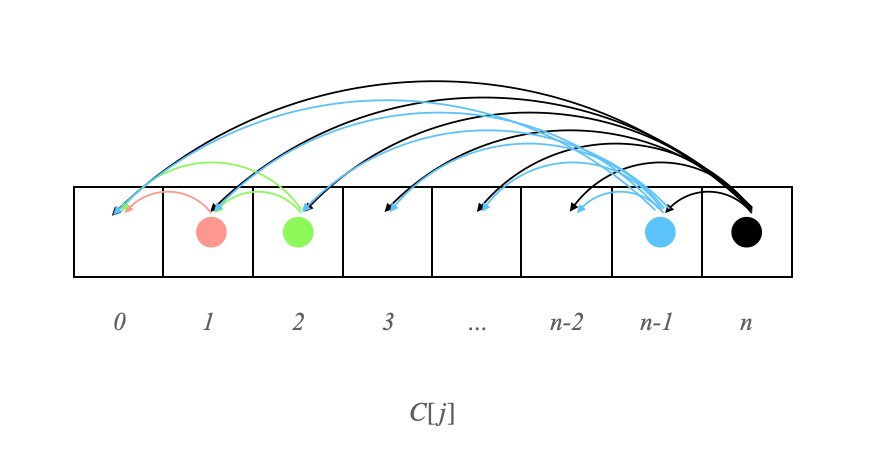
\includegraphics[scale=0.85]{./hw6q5.png}

\item Compute the value of an optimal solution bottom-up:

\begin{algorithmic}[1]
\Function{PrettyPrint}{$W$, $M$}
	\State $n = W.$length
	\State let $C[0..n]$ and $S[0..n]$ be new arrays of zeros \Comment{table initializations}
	\State let $A[0..n]$ be a new array of zeros  \Comment{$A$ is for accumulating words length}
	\For {$i = 1$ to $n$}
		\State $A[i] = A[i-1] + W[i]$.length
	\EndFor
	\For {$j = 1$ to $n$}
		\State $C[j] = +\infty$
		\For {$i = 0$ to $j - 1$}
			\State $t = M - (A[j] - A[i] + j - (i + 1))$ \Comment{trailing spaces after fitting $w_{i+1}$ to $w_j$ on a line}
			\If {$t \ge 0$}
				\If {$j == n$}
					\State $\textit{cost} = C[i]$
				\Else
					\State $\textit{cost} = C[i] + t^3$
				\EndIf
				\If {$\textit{cost} < C[j]$}
					\State $C[j] = \textit{cost}$
					\State $S[j] = i$
				\EndIf
			\EndIf
		\EndFor
	\EndFor
	\State \textbf{return} $C$, $S$
\EndFunction
\end{algorithmic}

\item Trace the optimal solution from the computed information:
\begin{algorithmic}[1]
\Function{Trace}{$W$, $S$}
	\State $i = S.$lastElem \Comment{this is the index of the last word on the second to last line}
	\State $E = [W.\text{length}, i]$ 
	\While {$S[i] > 0$}
		\State $i = S[i]$ \Comment{$i$ is updated to the index of the last word on the line prior to $w_i$}
		\State $E.$push($i$)
	\EndWhile
	\State $\textit{start} = 1$
	\For {$e$ in \textproc{\textsc{Reversed}}$(E)$}
		\State \textproc{\textsc{Print}}(" ".join($W[\textit{start}: e]$)) \Comment{join words by spaces in between}
		\State $\textit{start} = e$
	\EndFor
\EndFunction
\end{algorithmic}

\item Runtime and space requirements:

The for loop at line 5 in $\textproc{\textsc{PrettyPrint}}$ runs in $O(n)$-time to facilitate computing trailing spaces. The doubly-nested for loops in $\textproc{\textsc{PrettyPrint}}$ runs $1 + 2 + ... + (n - 1) + n$ iterations. In each iteration there is constant amount of work to do. Overall, the function runs in $O(n^2)$-time to produce $C$ and $S$ tables. It uses $O(n)$-space for storing the one-dimensional $C$, $S$, and $A$ arrays. The function $\textproc{\textsc{Trace}}$ runs in time linear to the number of lines in the final pretty print. In the worst case, it's bounded by $O(n)$ assuming every word is on a separate line. With the same reasoning, it uses $O(n)$-space to store $E$. Overall, the algorithm runs in $O(n^2)$-time and takes $O(n)$-space.

\end{enumerate}



\end{document}